\chapter{Tecnologias Utilizadas}
\section{\textit{Frameworks web}}

É comum, em desenvolvimento de sistemas, usar soluções prontas como forma de simplificar o desenvolvimento de soluções mais avançadas. Em especial, na área de aplicações \textit{web}, é uma solução desejável pois além de acelerar o desenvolvimento, usa-se uma solução amplamente testada no mercado e de confiança para aplicações comerciais. Tais soluções prontas são chamadas de arcabouços (ou \textit{frameworks}). Para este projeto, não foi diferente: por motivos de agilidade, mesclados com requisitos de manutenibilidade do sistema, foi escolhido um \textit{framework} em linguagem Python, chamado \textbf{Django}.

\subsection{Django}
O Django teve sua primeira versão lançada em Setembro de 2008\cite{djangowikispaces2012}, contendo muito do que é encontrado atualmente na versão 2.1\cite{djangodocs}: padrão \textit{Model-View-Controller}, gerenciamento de banco de dados eficiente, padrões para roteamento de URLs, entre outras funcionalidades. O \textit{framework} nasceu de uma empresa de desenvolvimento de sistemas para jornalismo, onde os prazos são frequentes e, muitas vezes, inegociáveis, logo, surgiu uma necessidade de uma solução rápida de implementar e estável para aplicações comerciais, resultando no nascimento do Django\cite{djangogeneral2018}.

O Django é estruturado em aplicações (apps), onde cada aplicação corresponde a uma parte do sistema, geralmente independente e reciclável (ou seja, pode ser usada em aplicações Django diferentes). Cada aplicação segue o padrão \textit{Model-View-Controller}, que será explicado melhor adiante\cite{djangodocs}. Hoje, sua versão mais recente estável é a 2.1, que corrigiu algumas novidades da versão 2.0. É esta versão que foi usada pelo projeto em questão, dado que é estável e possui suporte de apoio da equipe até Dezembro de 2020\cite{djangodownload}.

\subsection{Padrão \textit{Model-View-Controller}}
O padrão \textit{Model-View-Controller} - MVC (ou \textit{Model-Template-View} - MTV) consiste em um padrão arquitetural de software para organizar os componentes da aplicação de maneira eficiente e de fácil manutenção. Há diversos outros padrões arquiteturais (como por exemplo a arquitetura em camadas), mas o caso do Django é explícito o uso desse padrão.

Este padrão é dividido em três grandes grupos\cite{thedjangobook2018}:

\begin{itemize}
    \item Modelo (\textit{Model}): Uma representação (interface) para os dados da aplicação.
    \item Visualização (\textit{View}): Camada de apresentação dos dados da aplicação. No caso do Django, está mais alinhado com o \textit{Template}.
    \item Controlador (\textit{Controller}): Camada de controle que interliga o modelo com a apresentação dos dados, onde geralmente fica a lógica de negócio. No caso do Django, está mais alinhado com a \textit{View}.
\end{itemize}

\begin{figure}[H]
    \centering
    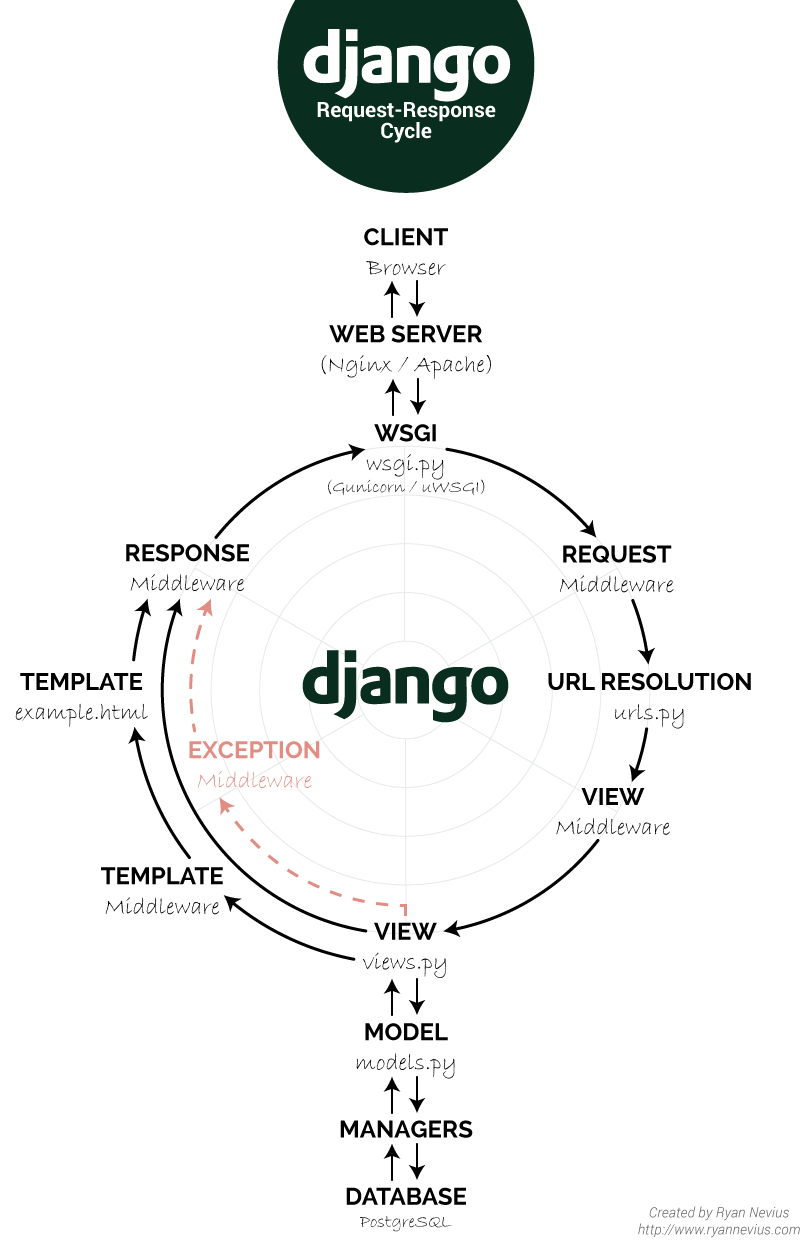
\includegraphics[scale=0.20]{model-view-template.png}
    \caption{Arquitetura MTV do Django\cite{codelv2018}}
    \label{fig:mtv-django}
\end{figure}

A vantagem do padrão está no fluxo de dados evidente que existe entre as camadas, além de evitar códigos com funcionalidades diferentes em lugares errados, como por exemplo lógica de negócio na camada de apresentação.

\section{Banco de Dados}

Assim como em projetos grandes de sistemas, o uso de banco de dados tornou-se necessário no projeto em questão. Porém, hoje possuímos diversos tipos e estruturas de bancos de dados distintos e, de acordo com os requisitos de um projeto, é tomada a decisão de qual é o melhor banco a ser usado no contexto. Segundo a definição traduzida do dicionário de Cambridge\cite{cambridgeuniversitypress2018}, o significado comercial de Banco de Dados é:

\begin{citacaoLonga}
Um sistema de computador que contém uma grande quantidade de informações que podem ser visualizadas ou alteradas facilmente.
\end{citacaoLonga}

Essencialmente, um banco de dados é uma coleção de informações organizadas, estruturadas ou não, guardadas em um computador e usadas para os mais diversos fins. Para acessar essas informações, usam-se sistemas para controlar a consulta a essas informações, tanto do lado do usuário final, como do lado dos desenvolvedores. Esses sistemas são conhecidos como Sistemas de Gerenciamento de Banco de Dados (SGBD)\cite{devmedia2014}.

Há diversos tipos de banco de dados no mercado, porém, para o projeto, foi adotado o modelo clássico relacional.

\subsection{Bancos Relacionais}
Bancos de dados relacionais são bancos onde cada coletânea de dados pode possuir uma relação pré-estabelecida. Para isso, é comum a estruturação deles por meio de tabelas, onde cada coluna é um tipo de dado e a linha é o valor em si. Cada linha é marcada com o que é chamado de chave primária, e é por meio dela que é possível fazer referência desse dado em outras tabelas. Para auxiliar as consultas e operações nesses bancos, bancos relacionais costumam usar uma linguagem própria para realizar tais operações, conhecida como Linguagem de Consulta Estruturada (Structured Query Language - SQL). O SQL foi determinado como padrão em 1986 e, desde então, é usado com pequenas variações entre os mais diversos mecanismos de banco de dados relacionais\cite{amazonwebservices2018}.

\subsubsection{SQLite}
O SQLite é um SGBD implementado em C, com o diferencial de ser leve e embutido na própria aplicação, ou seja, o banco fica junto com a aplicação carregada. A principal vantagem está em sua simplicidade, dado que o banco praticamente está pronto para ser usado pelo sistema. A desvantagem está no acoplamento entre o banco e a aplicação, o que nem sempre é saudável\cite{devmedia2007}.

\subsubsection{PostgreSQL}
O PostgreSQL é outro tipo de SGBD, bem mais robusto que o exemplo anterior, dado que é um servidor real dedicado para realizar a gestão de dados. Ele é mais preparado para lidar com cargas de trabalho maiores, consultas mais pesadas, entre outras tarefas robustas. Além disso, possui uma segurança mais reforçada, técnicas de recuperação de dados, entre outros. Como principal desvantagem, temos a complexidade para configurar e manter esse banco como infraestrutura dependente do projeto, o que, em casos de projetos simples, pode ser trabalho desnecessário\cite{devmedia2015}.

\subsection{Decisões de Projeto}
No âmbito de banco de dados relacional, o Django usa como padrão o SQLite, o que atendeu bem durante o desenvolvimento. Já o Heroku tem como banco de dados padrão o PostgreSQL, o que exigiu o chaveamento entre os bancos no ambiente local de desenvolvimento e os ambientes de validação hospedados no serviço. Por isso, o projeto possui configurado dois pacotes de gerenciamento de banco de dados, um para SQLite (nativo do Django), outro para PostgreSQL (o Psycopg\cite{lucassouto2017}).

\section{Ambientes de Validação}
É uma boa prática, para desenvolvimento de sistemas, criar diversos ambientes de aplicação, para validar as funcionalidades desenvolvidas tanto com a equipe de desenvolvimento, como com os \textit{stakeholders}, fora o ambiente onde a aplicação será hospedada, de fato (ou seja, onde ela ficará em ambiente de produção). Cada sistema exige 1 ou mais ambientes durante o fluxo de desenvolvimento, de acordo com a complexidade de negócios do projeto. Durante este capítulo, será explicitado mais sobre como foi estruturado os ambientes de teste e quais tecnologias de apoio foram usadas.

\subsection{Organização Genérica}
Para o projeto, foram organizados três ambientes de aplicação para realizar os processos de validação e homologação do sistema, para permitir testes isolados dos \textit{stakeholders} sem afetar o fluxo de desenvolvimento. São eles: Desenvolvimento (ou \textit{next-release}), Homologação (ou \textit{staging}) e Produção (ou \textit{production})\cite{ilyasabanin2018}.

\subsubsection{Desenvolvimento}
No ambiente de desenvolvimento, sempre fica a versão mais recente e estável da aplicação, com as novas funcionalidades desenvolvidas e testadas já integradas no ambiente. Essa versão serve como uma prévia do que será entregue para homologação. As mudanças nesse ambiente são mais frequentes, dado que uma nova funcionalidade completa já pode ir para este ambiente.

\subsubsection{Homologação}
Já neste ambiente, as mudanças são bem menores e servem como ambiente de aprovação dessas mudanças por parte dos \textit{stakeholders}. No caso do sistema de TCCs, ele serviu como homologação com os coordenadores do curso. Se possível, ele deve ser o mais fiél ao ambiente final de produção, assim o comportamento ideal dele em homologação será o mesmo em produção.

\subsubsection{Produção}
Já este ambiente é onde o sistema irá rodar, de fato. Esse ambiente deve ser o mais estável possível, com alterações apenas homologadas pelos \textit{stakeholders}. Salvo raras exceções, como falhas e problemas encontrados, nada deve ser colocado aqui sem a aprovação no ambiente de homologação.

\begin{figure}[H]
    \centering
    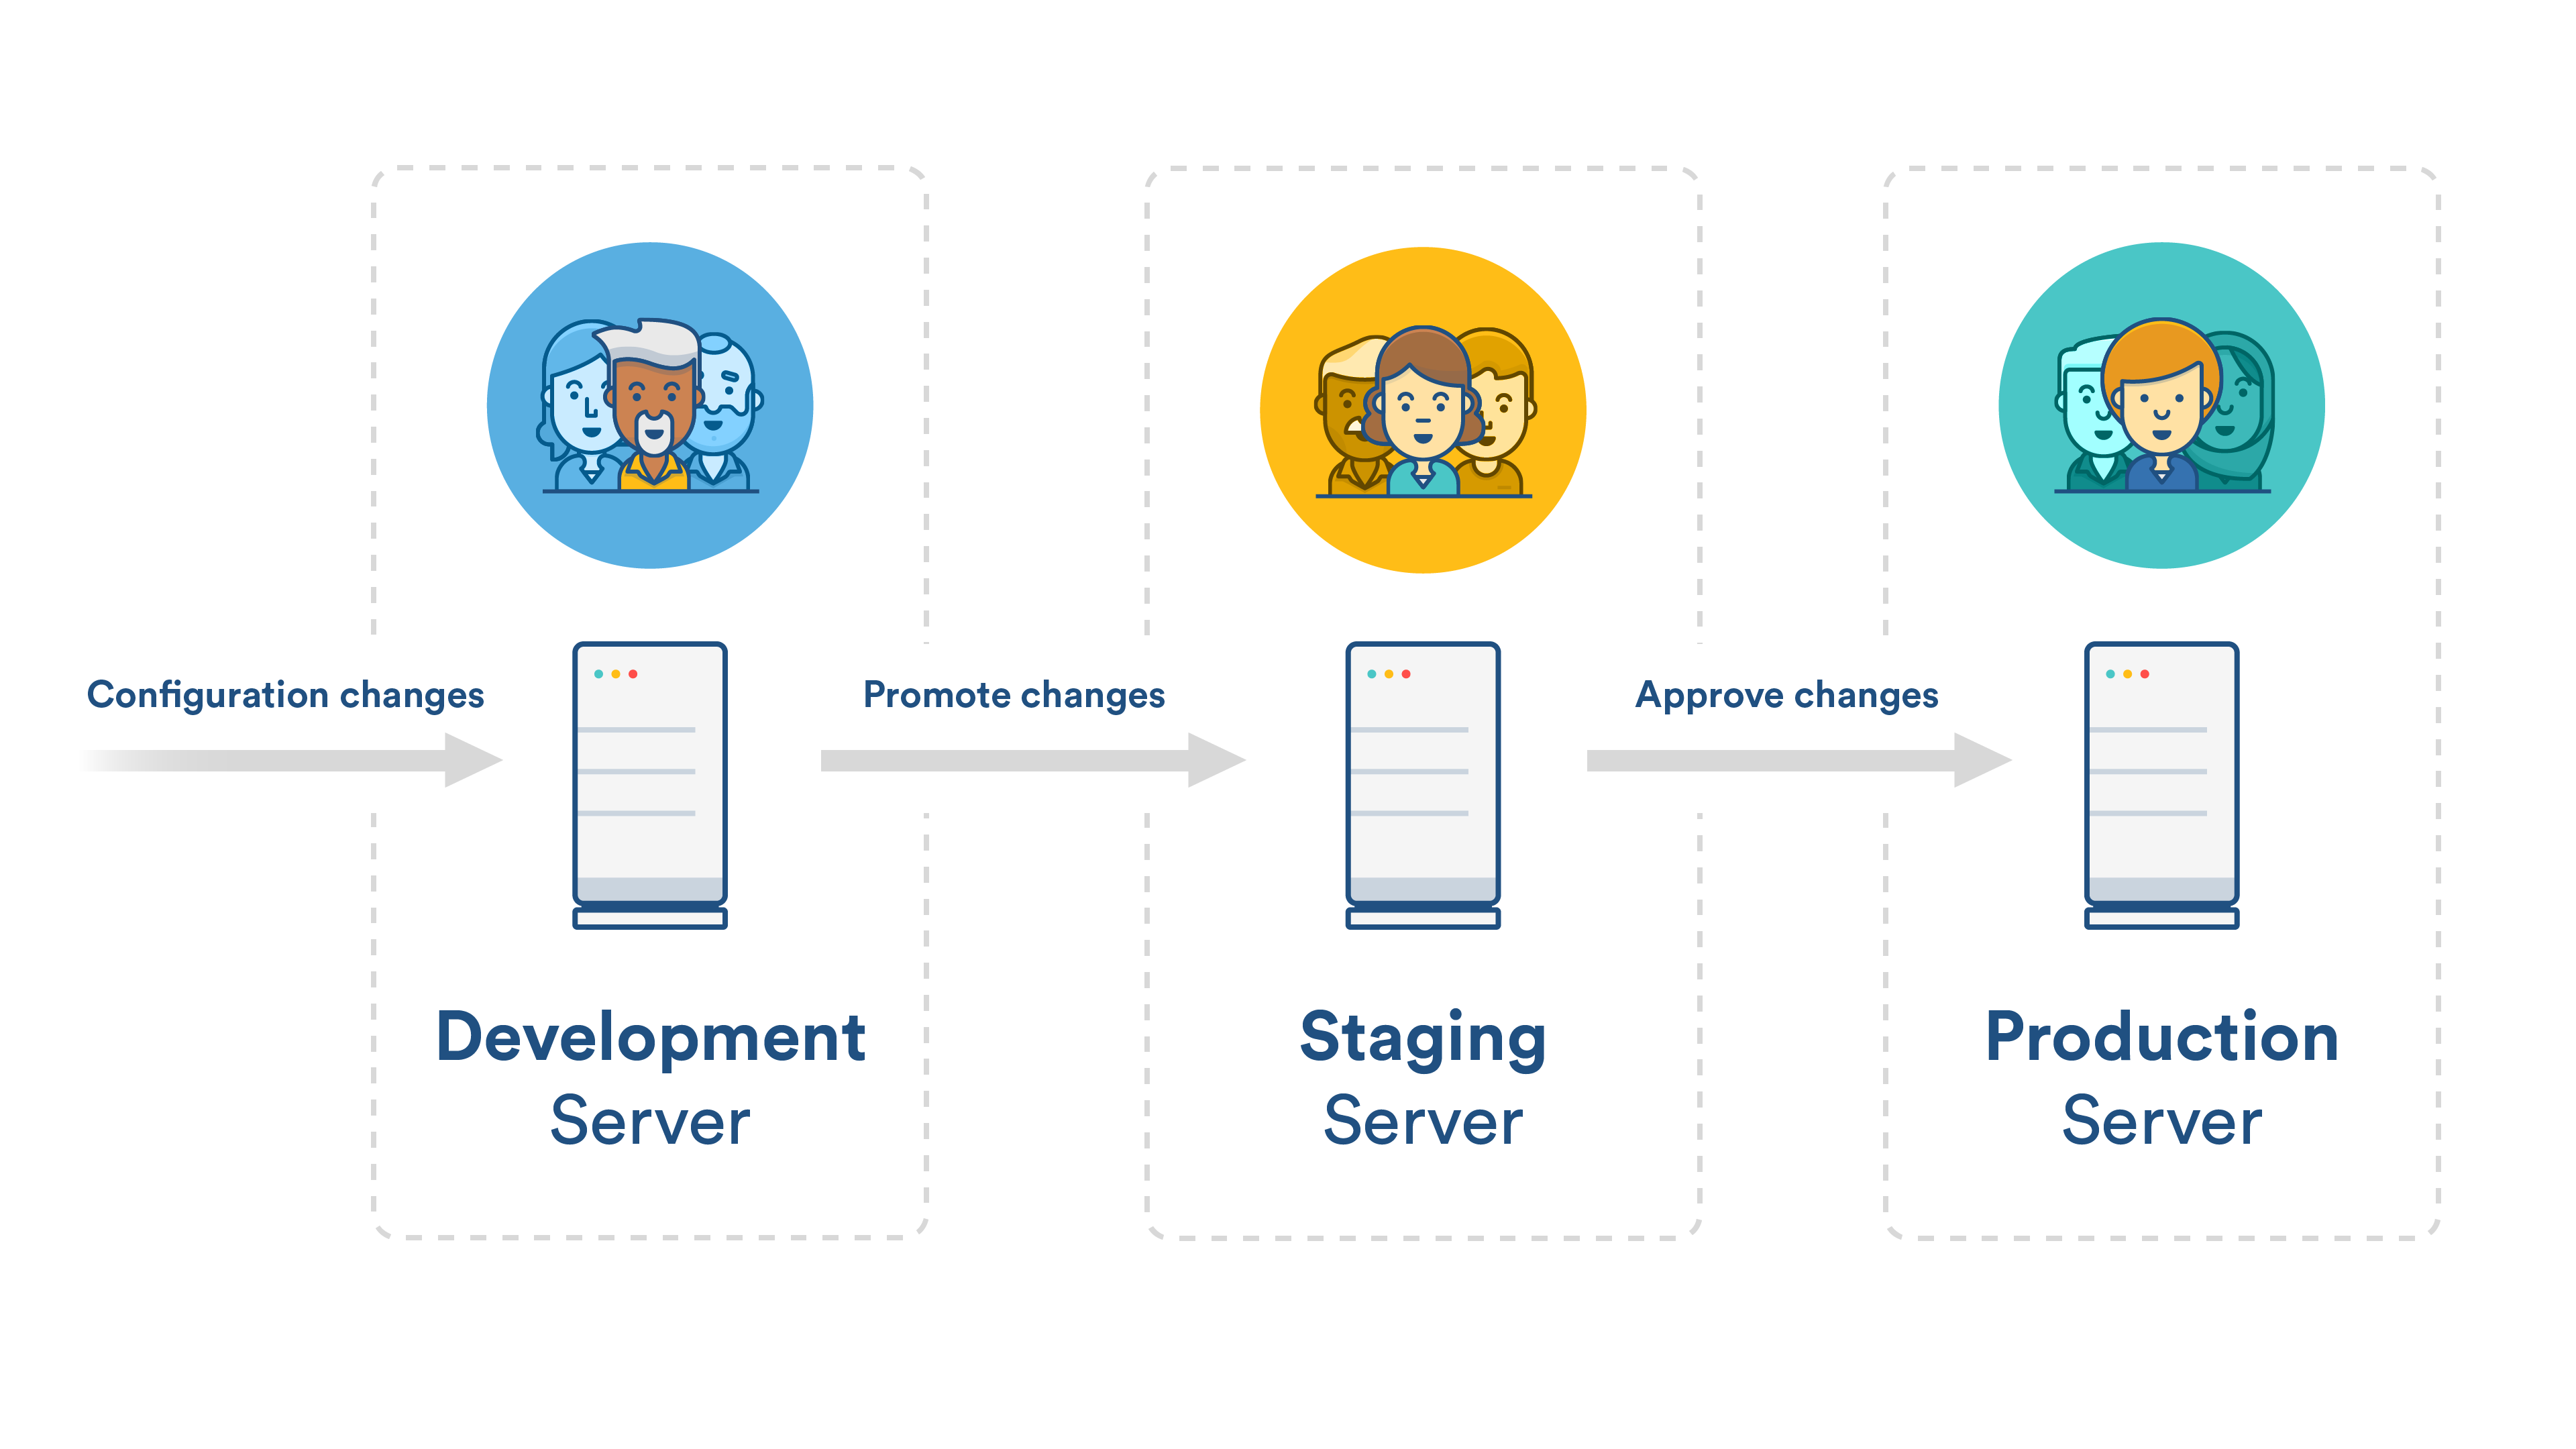
\includegraphics[scale=0.15]{software-flow.png}
    \caption{Fluxo do Sistema em Desenvolvimento\cite{atlassiansupport2018}}
    \label{fig:software-flow}
\end{figure}

\subsection{Estruturação no Projeto}
Para o projeto, foram construídos dois ambientes remotos, fora o ambiente final de produção que deve ficar na nuvem da USP. Os ambientes de desenvolvimento e homologação foram criados no Heroku, um serviço de plataforma (\textit{Platform as a Service} - \textbf{PaaS}), com os seguintes domínios:

\begin{itemize}
    \item Desenvolvimento: \href{https://tccapp-next-release.herokuapp.com}{https://tccapp-next-release.herokuapp.com}
    \item Homologação: \href{https://tccapp-staging.herokuapp.com}{https://tccapp-staging.herokuapp.com}
\end{itemize}

\section{Tecnologia Usada: Heroku\cite{lucasarthurfelgueiras2018}}

O Heroku é uma plataforma de computação em nuvem conhecida no mercado, com a possibilidade de subir aplicações nas linguagens Ruby, Node.js, Java, Python, Clojure, Scala, Go e PHP. O grande destaque do Heroku está na facilidade em subir uma aplicação com facilidade e de maneira gratuita, o que possibilita testar e validar ideias básicas antes de escalar de fato. A estrutura básica do Heroku funciona com o uso de \textit{dynos}, que servem tanto para hospedar sua aplicação principal quanto máquinas auxiliares para serviços externos e/ou paralelos.

\subsection{Funcionamento básico}

\begin{figure}[H]
  \centering
  \includegraphics[scale=0.20]{heroku-architecture.eps}
  \caption{Arquitetura Básica do Heroku\cite{safariheroku}}
  \label{fig:heroku-architecture}
\end{figure}

O funcionamento do Heroku consiste no uso de \textit{dynos} para hospedar as aplicações e nos \textit{routers} para tratar e encaminhas as requisições dos usuários. Além disso, o próprio Heroku disponibiliza extensões para gerenciar sua aplicação, como por exemplo o gerenciador de IP estático, ou o banco de dados necessário para a aplicação.

\subsection{Tarifação}

O Heroku possui um diferencial em relação à tarifação: possui um plano básico gratuito que possibilita testar aplicações de maneira fácil e sem dificuldades de expansão. Essencialmente, a cobrança do Heroku ocorre via uso de seus \textit{dynos}-hora. Além disso, há a cobrança pelas extensões usadas dentro da aplicação, onde, no geral, há um plano gratuito de testes ou até para projetos pequenos funcionarem com tranquilidade sem necessidades de escalabilidade.
